\documentclass[12pt]{article}
\usepackage{fullpage}
\usepackage{times}
\usepackage{float}
\usepackage[normalem]{ulem}
\usepackage{fancyhdr,graphicx,amsmath,amssymb, mathtools, scrextend, titlesec, enumitem}
\usepackage[ruled,vlined]{algorithm2e} 
\include{pythonlisting}

\title{Dense Neural Networks}
\author{Tadeu Silva (Deds)}
\begin{document}
\maketitle

\begin{figure}[H]
    \centering
    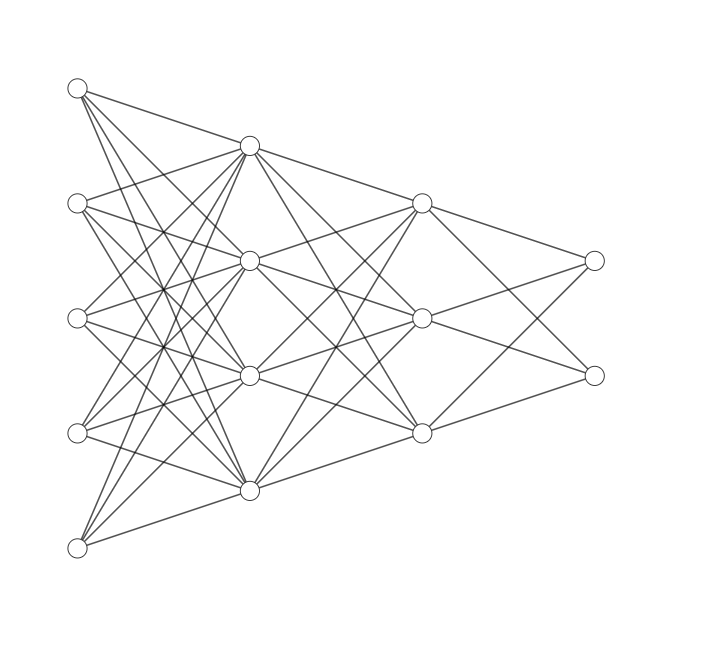
\includegraphics[width=0.9\linewidth]{images/NN.png}
    \caption{Architecture of Neural Network}
    \label{fig1}
\end{figure}   

\newpage

\section{Introduction}
A Neural Network is made by two steps: \textbf{Forward} pass and \textbf{Backward} pass. In the Forward pass, the next layer is a linear transformationa between the previous one, with an activation function in the end of each result. In the Backward pass, we asses the \textbf{loss} (how our prediction is wrong from the actual data) and update the parameters (weights and bias) according to an \textbf{Optimizer} (in this case Gradient Descent).


\begin{figure}[H]
    \centering
    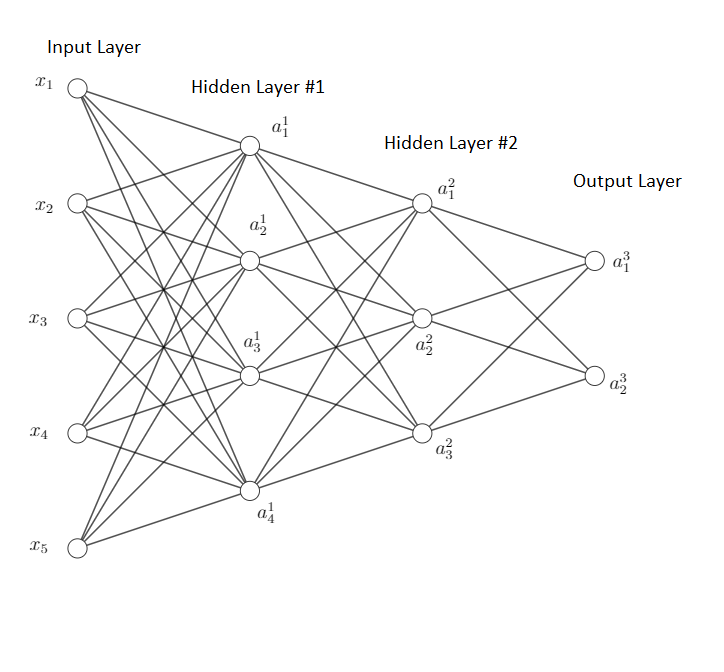
\includegraphics[width=0.79\linewidth]{images/NN_info.png}
    \caption{Dense Neural Network: Activation}
    \label{fig2}
\end{figure}   


\section{Forward Pass}

Given an input $\overrightarrow{x}$ in the Input Layer, the Hidden Layer \#1 has output:
\begin{equation}
    z^{1} = W^{1} \cdot \overrightarrow{x} + b^{1}
\end{equation}
where $W$ is the \textbf{Weights} matrix, $b$ is the \textbf{bias} vector and $\overrightarrow{x}$ is the \textbf{output} vector.
\\
Obs:
\begin{itemize}
    \item $\overrightarrow{x}$ is a $(m,1)$ vector
    \item $W$ is a $(n,m)$ matrix
    \item $b$ is a $(n,1)$ matrix
\end{itemize}

Then we \textbf{activate} the next layer by an Activation Funtion, to simulate nonlinear behavior (otherwise we are only doing linear regression). The final result for the next layer is:
\begin{equation}
    a^{1} = \sigma (z^{1}) = \sigma ( W^{1} \cdot \overrightarrow{x} + b^{1} )
\end{equation}
\textbf{Obs}: The input is called $\overrightarrow{x}$ , but the other layers are called \textbf{a}

So, in general, the activation of layer l is given by:
\begin{equation}
    a^{l} = \sigma (z^{l}) = \sigma ( W^{l} \cdot a^{l-1} + b^{l} )
\end{equation}

\subsection{Example}

In our example at figure \ref{fig2} we have:
\\
\textbf{Hidden Layer \# 1}
\begin{equation}
\begin{bmatrix}
a_{1}^{1}\\
a_{2}^{1}\\
a_{3}^{1}\\
a_{4}^{1}
\end{bmatrix}
=
\sigma
\left(
\begin{bmatrix}
z_{1}^{1}\\
z_{2}^{1}\\
z_{3}^{1}\\
z_{4}^{1}
\end{bmatrix}
\right)
=
\sigma
\left(
\begin{bmatrix}
x_{1}\\
x_{2}\\
x_{3}\\
x_{4}\\
x_{5}
\end{bmatrix}
\cdot
\begin{bmatrix}
W_{11}^{1} & W_{12}^{1} & W_{13}^{1} & W_{14}^{1} & W_{15}^{1} \\
W_{21}^{1} & W_{22}^{1} & W_{23}^{1} & W_{24}^{1} & W_{25}^{1} \\
W_{31}^{1} & W_{32}^{1} & W_{33}^{1} & W_{34}^{1} & W_{35}^{1} \\
W_{41}^{1} & W_{42}^{1} & W_{43}^{1} & W_{44}^{1} & W_{45}^{1} 
\end{bmatrix}
 +
 \begin{bmatrix}
b_{1}^{1}\\
b_{2}^{1}\\
b_{3}^{1}\\
b_{4}^{1}
\end{bmatrix}
\right)
\end{equation}
\\
\textbf{Hidden Layer \# 2}
\begin{equation}
\begin{bmatrix}
a_{1}^{2}\\
a_{2}^{2}\\
a_{3}^{2}
\end{bmatrix}
=
\sigma
\left(
\begin{bmatrix}
z_{1}^{2}\\
z_{2}^{2}\\
z_{3}^{2}
\end{bmatrix}
\right)
=
\sigma
\left(
\begin{bmatrix}
a_{1}^{1}\\
a_{2}^{1}\\
a_{3}^{1}\\
a_{4}^{1}
\end{bmatrix}
\cdot
\begin{bmatrix}
W_{11}^{2} & W_{12}^{2} & W_{13}^{2} & W_{14}^{2} \\
W_{21}^{2} & W_{22}^{2} & W_{23}^{2} & W_{24}^{2} \\
W_{31}^{2} & W_{32}^{2} & W_{33}^{2} & W_{34}^{2} \end{bmatrix}
 +
 \begin{bmatrix}
b_{1}^{2}\\
b_{2}^{2}\\
b_{3}^{2}
\end{bmatrix}
\right)
\end{equation}


\textbf{Output Layer}
\begin{equation}
\begin{bmatrix}
a_{1}^{3}\\
a_{2}^{3}
\end{bmatrix}
=
\sigma
\left(
\begin{bmatrix}
z_{1}^{3}\\
z_{2}^{3}
\end{bmatrix}
\right)
=
\sigma
\left(
\begin{bmatrix}
a_{1}^{2}\\
a_{2}^{2}\\
a_{3}^{2}
\end{bmatrix}
\cdot
\begin{bmatrix}
W_{11}^{3} & W_{12}^{3} & W_{13}^{3} \\
W_{21}^{3} & W_{22}^{3} & W_{23}^{3} \\ 
\end{bmatrix}
 +
 \begin{bmatrix}
b_{1}^{3}\\
b_{2}^{3}
\end{bmatrix}
\right)
\end{equation}

\section{Backward Pass}
\subsection{Loss}
In the Backward pass, we first compute our \textbf{loss} (aka the error of our output) and average along the data, to get a measure of our total uncertainty. So:
\begin{equation}
    loss = (\dfrac{1}{n}) \sum_{i=0}^{n} loss(a_{i}^{2}, y_{i})
\end{equation}
where n is the dimension of the output layer.
One option is to use the \textbf{Mean Squared Error} as the loss. So in our example we have:
\begin{equation}
    loss = (\dfrac{1}{n}) \sum_{i=0}^{n} (a_{i}^{2} - y_{i})^{2}
\end{equation}

\subsection{Backpropagation}
The second part is to calculate how each weight and bias had influence in the loss. So we want to calculate:
\begin{equation}
\nabla C
=
\begin{bmatrix}
\dfrac{\partial C}{\partial W} \\\\
\dfrac{\partial C}{\partial b} 
\end{bmatrix}
\end{equation}
We do that using the Backpropagation (chain rule). Remembering from calculus, the derivative of a composite function $f(g(x))$ can be written as:
\begin{equation}
    \dfrac{df}{dx} = \dfrac{df}{dg} \dfrac{dg}{dx}
\end{equation}


Another thing that is going to be useful is remember how to calculate the derivative of matrices. So, given a scalar function C (even do our loss depends of \textbf{y} and \textbf{a}, we can treat it as scalar), the derivative with respect to the matrix W, is given by:
\\\\
\begin{equation}
\dfrac{\partial C}{\partial W}
=
\begin{pmatrix}
\dfrac{\partial C}{\partial W_{11}} & \dfrac{\partial C}{\partial W_{12}} & \cdots & \dfrac{\partial C}{\partial W_{1m}} \\
\vdots & \vdots & \ddots & \vdots \\
\dfrac{\partial C}{\partial W_{n1}} & \dfrac{\partial C}{\partial W_{n2}} & \cdots & \dfrac{\partial C}{\partial W_{nm}} \\
\end{pmatrix}
\end{equation}

Similarly to the bias b:

\begin{equation}
\dfrac{\partial C}{\partial b}
=
\begin{pmatrix}
\dfrac{\partial C}{\partial b_{1}} \\
\vdots  \\
\dfrac{\partial C}{\partial b_{n}} 
\end{pmatrix}
\end{equation} 
\mbox{} \\

Following that same logic, we have $a(z(W))$, then we start from the Output layer and go backwards to the Input layer, as follows:

\begin{equation}
    \dfrac{\partial C}{\partial W} = \left( \dfrac{\partial C}{\partial a}\right) \left( \dfrac{\partial a}{\partial z}\right) \left(\dfrac{\partial z}{\partial W} \right)
\end{equation}
\begin{equation}
    \dfrac{\partial C}{\partial b} = \left( \dfrac{\partial C}{\partial a}\right) \left( \dfrac{\partial a}{\partial z}\right) \left(\dfrac{\partial z}{\partial b} \right)
\end{equation} \mbox{} \\

For the \underline{third} term, note that:

\[
z^{l} = W^{l}\cdot a^{l-1} + b^{l} \Rightarrow  \dfrac{\partial z^{l}}{\partial W^{l}} = a^{l-1}
\]
\[
z^{l} = W^{l}\cdot a^{l-1} + b^{l} \Rightarrow  \dfrac{\partial z^{l}}{\partial b^{l}} = 1
\] \mbox{} \\



For the \underline{second} term:
\[
\dfrac{\partial a}{\partial z} = \dfrac{d \sigma}{\partial z}
\] \mbox{} \\

The activation function $\sigma$ depends on the problem at hand. But let's suppose we are at a \textbf{classification} problem, so we'll go with the \textbf{Softmax} function, defined as:

\begin{equation}
    \sigma (z) = \dfrac{e^{z}}{\sum_{j=0}^{n} e^{z_{j}}}
\end{equation}

So the equation is:

\[
\dfrac{\partial a^{l}}{\partial z^{l}} = \dfrac{d \sigma}{\partial z^{l}} = z^{l} ( 1 - z^{l} )
\] \mbox{} \\

For the \underline{first} term, we have two options: 
 
\paragraph{1. Output Layer} \mbox{} \\
For the Output Layer, we just have the loss as our main metric. So the equation is:

\[
\dfrac{\partial C}{\partial a} = \dfrac{d loss}{da}
\]

In our example loss is \textbf{MSE}, so:

\[
\dfrac{\partial C}{\partial a^{2}} = 2(a_{2}^{2} - y_{i})
\]

\paragraph{2. Other Layers}  \mbox{} \\
In other layers, we have $a^{l} = a^{l+1}(z^{l+1}(a^{l}))$ \mbox{} \\
This means that the error in the layer l influences the error of layer l+1, and that's why the chain rule is so powerfull in keeping track of those links. So the equations goes as follows:

\[
\dfrac{\partial C}{\partial a^{l}} = \left(\dfrac{\partial C}{\partial a^{l+1}} \right)\left( \dfrac{\partial a^{l+1}}{\partial z^{l+1}}\right)\left( \dfrac{\partial z^{l+1}}{\partial a^{l}}\right)
\]

\subsubsection{Example}
Let's denote the following two operations:
\begin{itemize}
    \item $\times$ : element-wise multiplication, i.e. same dimensions only
    \item $\cdot$ : dot product, i.e (m,k) $\cdot$ (k,n) = (m,n)
\end{itemize}

This means that if:
\[
A =
\begin{bmatrix}
a_{11} & a_{12}\\
a_{21} & a_{22}
\end{bmatrix}
, B = 
\begin{bmatrix}
b_{11} & b_{12}\\
b_{21} & b_{22}
\end{bmatrix}
\Rightarrow
A X B = 
\begin{bmatrix}
a_{11}\cdot b_{11} & a_{12}\cdot b_{12}\\
a_{21}\cdot b_{21} & a_{22}\cdot b_{22}
\end{bmatrix}
\] 

Analogously, if:
\[
A =
\begin{bmatrix}
a_{11} & a_{12}\\
a_{21} & a_{22}
\end{bmatrix}
, B = 
\begin{bmatrix}
b_{11}\\
b_{21}
\end{bmatrix}
\Rightarrow
A \cdot B = 
\begin{bmatrix}
a_{11}\cdot b_{11} + a_{12}\cdot b_{21}\\
a_{21}\cdot b_{11} + a_{22}\cdot b_{21}
\end{bmatrix}
\] 



In our example at figure \ref{fig1} we have:
\\
\textbf{Output Layer - Weights}
\begin{equation}
    \dfrac{\partial C}{\partial W^{3}} = \left( \dfrac{\partial C}{\partial a^{3}}\right) \left( \dfrac{\partial a^{3}}{\partial z^{3}}\right) \left(\dfrac{\partial z^{3}}{\partial W^{3}} \right)
\end{equation}

\begin{equation}
\dfrac{\partial C}{\partial W^{3}}
= \Bigg[
2\left(
\begin{bmatrix}
a_{1}^{3} - y_{1}\\
a_{2}^{3} - y_{2}
\end{bmatrix}
\right)
\times
\begin{bmatrix}
z_{1}^{3} ( 1 - z_{1}^{3} )\\
z_{2}^{3} ( 1 - z_{2}^{3})
\end{bmatrix}
\Bigg]
\cdot
\left(
\begin{bmatrix}
a_{1}^{2}\\
a_{2}^{2}\\
a_{3}^{2}
\end{bmatrix}
\right)^{T}
\end{equation} 

\textbf{Output Layer - Bias}
\begin{equation}
    \dfrac{\partial C}{\partial b^{3}} = \left( \dfrac{\partial C}{\partial a^{3}}\right) \left( \dfrac{\partial a^{3}}{\partial z^{3}}\right)
\end{equation}

\begin{equation}
\dfrac{\partial C}{\partial b^{3}}
= 2\left(
\begin{bmatrix}
a_{1}^{3} - y_{1}\\
a_{2}^{3} - y_{2}
\end{bmatrix}
\right)
\times
\begin{bmatrix}
z_{1}^{3} ( 1 - z_{1}^{3} )\\
z_{2}^{3} ( 1 - z_{2}^{3})
\end{bmatrix}
\end{equation} \mbox{} \\

\textbf{Hidden Layer \# 2 - Weights}

\begin{equation}
    \dfrac{\partial C}{\partial W^{2}} = \left(\dfrac{\partial C}{\partial a^{2}}\right)\left( \dfrac{\partial a^{2}}{\partial z^{2}}\right) \left( \dfrac{\partial z^{2}}{\partial w^{2}}\right)
\end{equation}
where:
\begin{equation}
     \dfrac{\partial C}{\partial a^{2}} = \left( \dfrac{\partial C}{\partial a^{3}}\right) \left( \dfrac{\partial a^{3}}{\partial z^{3}}\right) \left(\dfrac{\partial z^{3}}{\partial a^{2}} \right)
\end{equation}

Note that:
\[
z^{3} = W^{3}\cdot a^{2} + b^{3} \Rightarrow \dfrac{\partial z^{3}}{\partial a^{2}} = W^{3}
\] 
So:
\begin{equation}
 \dfrac{\partial C}{\partial a^{2}}
=\Bigg(
\Bigg[
2\left(
\begin{bmatrix}
a_{1}^{3} - y_{1}\\
a_{2}^{3} - y_{2}
\end{bmatrix}
\right)
\times
\begin{bmatrix}
z_{1}^{3} ( 1 - z_{1}^{3} )\\
z_{2}^{3} ( 1 - z_{2}^{3})
\end{bmatrix}
\Bigg]^{T}
\cdot
\begin{bmatrix}
W_{11}^{3} & W_{12}^{3} & W_{13}^{3} \\
W_{21}^{3} & W_{22}^{3} & W_{23}^{3} \\ 
\end{bmatrix}
\Bigg)^{T}
\end{equation}

And finally:

\begin{equation}
\dfrac{\partial C}{\partial W^{2}} = \left(\dfrac{\partial C}{\partial a^{2}}\right)
\times
\begin{bmatrix}
z_{1}^{2} ( 1 - z_{1}^{2} )\\
z_{2}^{2} ( 1 - z_{2}^{2}) \\
z_{3}^{2} ( 1 - z_{3}^{2}) 
\end{bmatrix}
\Bigg]
\cdot
\left(
\begin{bmatrix}
a_{1}^{1}\\
a_{2}^{1}\\
a_{3}^{1}\\
a_{4}^{1}
\end{bmatrix}
\right)^{T}
\end{equation} \mbox{} \\

\textbf{Hidden Layer \# 2 - Bias}

\begin{equation}
\dfrac{\partial C}{\partial W^{2}} = \left(\dfrac{\partial C}{\partial a^{2}}\right)
\times
\begin{bmatrix}
z_{1}^{2} ( 1 - z_{1}^{2} )\\
z_{2}^{2} ( 1 - z_{2}^{2}) \\
z_{3}^{2} ( 1 - z_{3}^{2}) 
\end{bmatrix}
\end{equation} \mbox{} \\

\textbf{Hidden Layer \# 1 - Weights}

\begin{equation}
    \dfrac{\partial C}{\partial W^{1}} = \left(\dfrac{\partial C}{\partial a^{1}}\right)\left( \dfrac{\partial a^{1}}{\partial z^{1}}\right) \left( \dfrac{\partial z^{1}}{\partial w^{1}}\right)
\end{equation}
where:
\begin{equation}
     \dfrac{\partial C}{\partial a^{1}} = \left( \dfrac{\partial C}{\partial a^{2}}\right) \left( \dfrac{\partial a^{2}}{\partial z^{2}}\right) \left(\dfrac{\partial z^{2}}{\partial a^{1}} \right)
\end{equation} \mbox{} \\

Analogously as the Hidden Layer \# 2 we get the influence from every layer, starting from the output layer, remembering now that:

\[
z^{2} = W^{2}\cdot a^{1} + b^{2} \Rightarrow \dfrac{\partial z^{2}}{\partial a^{1}} = W^{2}
\] \mbox{} \\

So the final equation is:

\begin{equation}
\dfrac{\partial C}{\partial W^{1}} = \left(\dfrac{\partial C}{\partial a^{1}}\right)
\times
\begin{bmatrix}
z_{1}^{1} ( 1 - z_{1}^{1} )\\
z_{2}^{1} ( 1 - z_{2}^{1}) \\
z_{3}^{1} ( 1 - z_{3}^{1}) \\
z_{4}^{1} ( 1 - z_{4}^{1}) 
\end{bmatrix}
\Bigg]
\cdot
\left(
\begin{bmatrix}
x_{1}\\
x_{2}\\
x_{3}\\
x_{4}\\
x_{5}
\end{bmatrix}
\right)^{T}
\end{equation} \mbox{} \\

\textbf{Hidden Layer \# 1 - Bias}
\begin{equation}
\dfrac{\partial C}{\partial W^{1}} = \left(\dfrac{\partial C}{\partial a^{1}}\right)
\times
\begin{bmatrix}
z_{1}^{1} ( 1 - z_{1}^{1} )\\
z_{2}^{1} ( 1 - z_{2}^{1}) \\
z_{3}^{1} ( 1 - z_{3}^{1}) \\
z_{4}^{1} ( 1 - z_{4}^{1}) 
\end{bmatrix}
\end{equation} \mbox{} \\

\subsection{Optimizing}
For the last step, we optimize the weights accordingly to the changes calculated on the previous section. There are a few optimizers, but the two most used are: \textbf{SGD} (Stochastic Gradient Descent) and \textbf{Adam}.   \mbox{} \\

\paragraph{SGD - Stochastic Gradient Descent} \mbox{} \\
The SGD is based in the simple idea that: the gradient shows the growth direction. Because we want to \textbf{decrease} our error/loss, we simple get the opposite direction adding the minus sign. So the equation is:

\begin{equation}
    W^{l} = W^{l} - lr \times \dfrac{\partial C}{\partial W^{l}}
\end{equation}
\begin{equation}
    b^{l} = b^{l} - lr \times \dfrac{\partial C}{\partial b^{l}}
\end{equation}
where lr is the \textbf{learning rate}, a parameter $( lr < 0 )$ just to make sure that we don't make great jumps and `miss` the local minima.


Depending in the size of our data, we usually don't go through \textbf{every} data available through each iteration (usually called epochs). The Stochastic Gradient Descent takes a \textbf{batch} size, where we do the forward/backwards pass only in a sample of the data, to minimize computation costs.

\end{document}